\documentclass[tikz,border=22pt]{standalone}
\usepackage[T1]{fontenc}
\usepackage{helvet}
\renewcommand{\familydefault}{\sfdefault}
\usepackage{amsmath,amssymb}
\usetikzlibrary{calc,positioning,fit,backgrounds,shapes.geometric,shapes.symbols,arrows.meta,decorations.pathreplacing}

% =============================================================================
% CANONICAL MLSYSBOOK PALETTE
% =============================================================================
\definecolor{DarkSlate}{HTML}{0F172A}
\definecolor{slatesteel}{HTML}{334155}
\definecolor{BlueLine}{HTML}{006395}
\definecolor{BlueL}{RGB}{209,243,255}
\definecolor{BlueL0}{HTML}{F0F9FF}
\definecolor{GreenLine}{HTML}{008F45}
\definecolor{GreenL}{RGB}{219,253,166}
\definecolor{GreenL0}{HTML}{EBF8F2}
\definecolor{forestsage}{HTML}{166534}
\definecolor{OrangeLine}{HTML}{E67817}
\definecolor{OrangeL}{RGB}{254,237,222}
\definecolor{OrangeL0}{HTML}{FFFBEB}
\definecolor{warmochre}{HTML}{92400E}
\definecolor{RedLine}{HTML}{D9534F}
\definecolor{RedL}{RGB}{253,226,240}
\definecolor{RedL0}{HTML}{FEF2F2}
\definecolor{deepburgundy}{HTML}{991B1B}
\definecolor{VioletLine}{HTML}{7E317B}
\definecolor{VioletL}{RGB}{247,215,247}
\definecolor{amethyst}{HTML}{581C87}
\definecolor{amethystL0}{HTML}{FAF5FF}
\definecolor{GrayLine}{HTML}{64748B}
\definecolor{coolparchment}{HTML}{F8FAFC}
\definecolor{CardBorder}{HTML}{CBD5E1}
\definecolor{ChipBlack}{HTML}{181F2C}
\definecolor{GoldPin}{HTML}{EAB308}

\tikzset{
  >=Latex,
  font=\sffamily,
  flow_arrow/.style={->, >=Latex, line width=1.1pt},
  flow_arrow_thick/.style={->, >=Latex, line width=1.6pt},
  dram_node/.style={draw=slatesteel!60, fill=white, rounded corners=2pt, inner xsep=4pt, inner ysep=2.5pt, font=\fontsize{5.2pt}{6.4pt}\selectfont, minimum height=0.52cm, text width=3.0cm, align=left},
}

\begin{document}
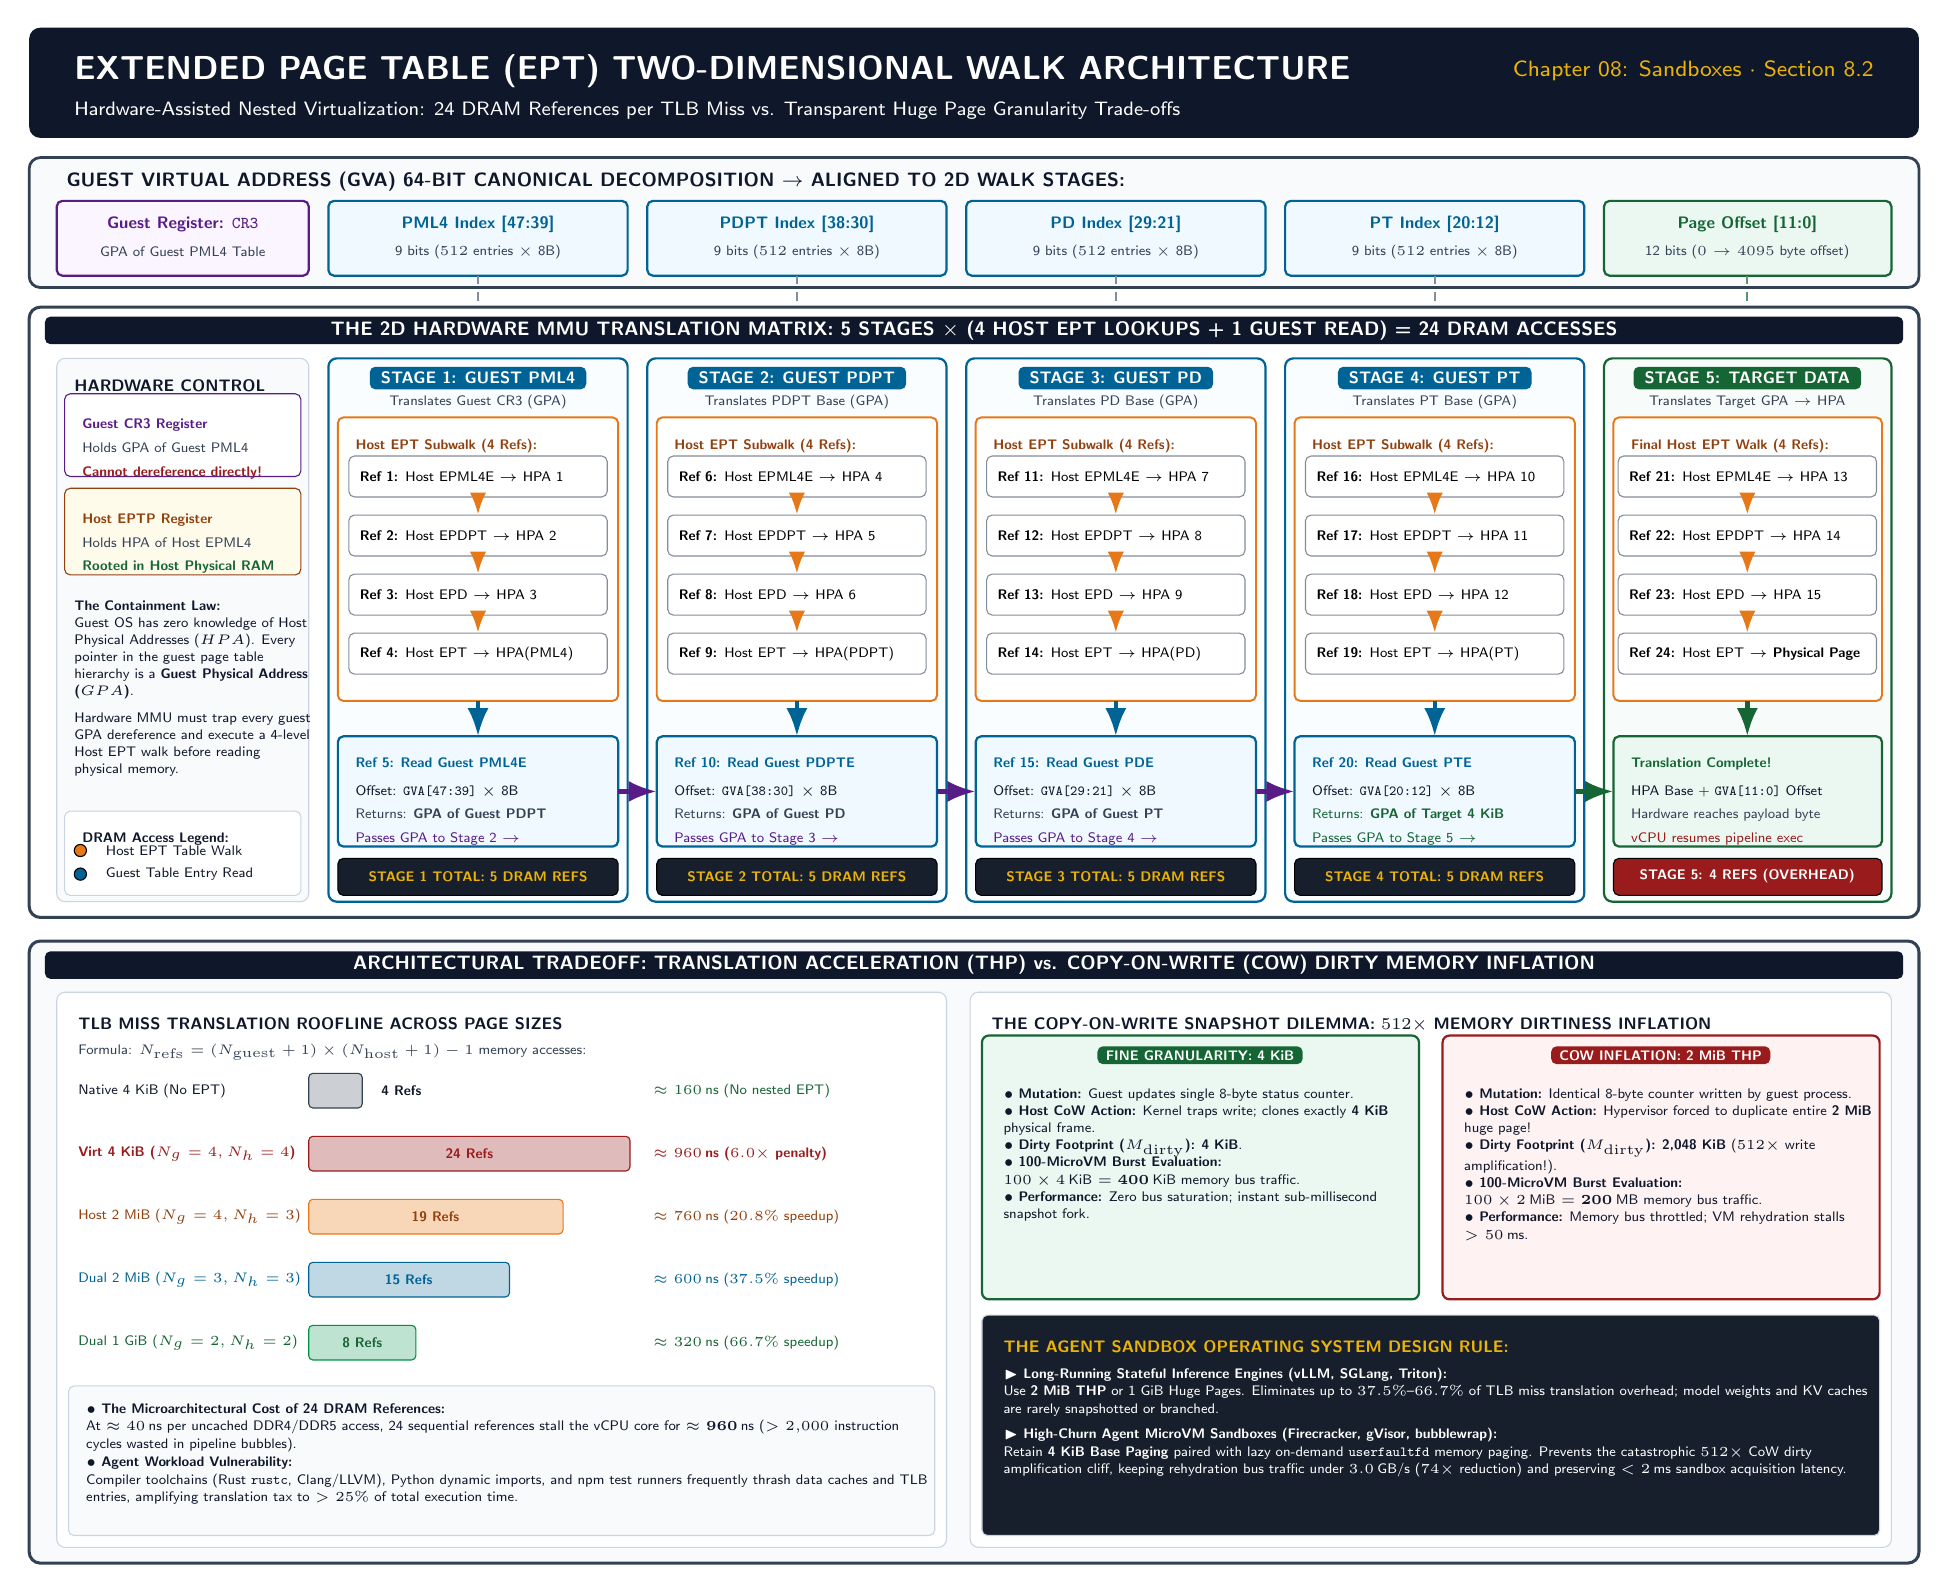
\begin{tikzpicture}[x=1cm, y=1cm]

% =============================================================================
% TOP TITLE BANNER (y: 18.6 to 20.0)
% =============================================================================
\draw[fill=DarkSlate, draw=none, rounded corners=4pt] (0, 18.6) rectangle (24.0, 20.0);
\node[anchor=west, font=\bfseries\large, text=white] at (0.45, 19.45) {
  EXTENDED PAGE TABLE (EPT) TWO-DIMENSIONAL WALK ARCHITECTURE
};
\node[anchor=east, font=\footnotesize, text=GoldPin] at (23.55, 19.45) {
  Chapter 08: Sandboxes $\cdot$ Section 8.2
};
\node[anchor=west, font=\scriptsize, text=white!85] at (0.45, 18.95) {
  Hardware-Assisted Nested Virtualization: 24 DRAM References per TLB Miss vs. Transparent Huge Page Granularity Trade-offs
};

% =============================================================================
% 1. TOP TIER: GUEST VIRTUAL ADDRESS (GVA) ALIGNED DECOMPOSITION (y: 16.7 to 18.35)
% =============================================================================
\draw[draw=slatesteel, fill=coolparchment, line width=1.0pt, rounded corners=4pt] (0, 16.7) rectangle (24.0, 18.35);

% Section Header
\node[anchor=west, font=\bfseries\fontsize{7pt}{8.5pt}\selectfont, text=DarkSlate] at (0.35, 18.05) {
  GUEST VIRTUAL ADDRESS (GVA) 64-BIT CANONICAL DECOMPOSITION $\to$ ALIGNED TO 2D WALK STAGES:
};

% Guest CR3 (GPA) Box (aligned with hardware control column)
\draw[draw=amethyst, fill=amethystL0, line width=0.8pt, rounded corners=2pt] (0.35, 16.85) rectangle (3.55, 17.8);
\node[font=\bfseries\fontsize{6.2pt}{7.2pt}\selectfont, text=amethyst] at (1.95, 17.5) {Guest Register: \texttt{CR3}};
\node[font=\fontsize{5.2pt}{6.2pt}\selectfont, text=slatesteel] at (1.95, 17.15) {GPA of Guest PML4 Table};

% PML4 Index Box (aligned with Stage 1)
\draw[draw=BlueLine, fill=BlueL0, line width=0.8pt, rounded corners=2pt] (3.80, 16.85) rectangle (7.60, 17.8);
\node[font=\bfseries\fontsize{6.5pt}{7.5pt}\selectfont, text=BlueLine] at (5.70, 17.5) {PML4 Index [47:39]};
\node[font=\fontsize{5.2pt}{6.2pt}\selectfont, text=slatesteel] at (5.70, 17.15) {9 bits ($512$ entries $\times$ 8B)};

% PDPT Index Box (aligned with Stage 2)
\draw[draw=BlueLine, fill=BlueL0, line width=0.8pt, rounded corners=2pt] (7.85, 16.85) rectangle (11.65, 17.8);
\node[font=\bfseries\fontsize{6.5pt}{7.5pt}\selectfont, text=BlueLine] at (9.75, 17.5) {PDPT Index [38:30]};
\node[font=\fontsize{5.2pt}{6.2pt}\selectfont, text=slatesteel] at (9.75, 17.15) {9 bits ($512$ entries $\times$ 8B)};

% PD Index Box (aligned with Stage 3)
\draw[draw=BlueLine, fill=BlueL0, line width=0.8pt, rounded corners=2pt] (11.90, 16.85) rectangle (15.70, 17.8);
\node[font=\bfseries\fontsize{6.5pt}{7.5pt}\selectfont, text=BlueLine] at (13.80, 17.5) {PD Index [29:21]};
\node[font=\fontsize{5.2pt}{6.2pt}\selectfont, text=slatesteel] at (13.80, 17.15) {9 bits ($512$ entries $\times$ 8B)};

% PT Index Box (aligned with Stage 4)
\draw[draw=BlueLine, fill=BlueL0, line width=0.8pt, rounded corners=2pt] (15.95, 16.85) rectangle (19.75, 17.8);
\node[font=\bfseries\fontsize{6.5pt}{7.5pt}\selectfont, text=BlueLine] at (17.85, 17.5) {PT Index [20:12]};
\node[font=\fontsize{5.2pt}{6.2pt}\selectfont, text=slatesteel] at (17.85, 17.15) {9 bits ($512$ entries $\times$ 8B)};

% Offset Box (aligned with Stage 5)
\draw[draw=forestsage, fill=GreenL0, line width=0.8pt, rounded corners=2pt] (20.00, 16.85) rectangle (23.65, 17.8);
\node[font=\bfseries\fontsize{6.5pt}{7.5pt}\selectfont, text=forestsage] at (21.82, 17.5) {Page Offset [11:0]};
\node[font=\fontsize{5.2pt}{6.2pt}\selectfont, text=slatesteel] at (21.82, 17.15) {12 bits ($0 \to 4095$ byte offset)};

% Subtle vertical dashed guide arrows linking GVA bitfields to Stages
\draw[flow_arrow, dashed, draw=slatesteel!60, line width=0.7pt] (5.70, 16.85) -- (5.70, 15.82);
\draw[flow_arrow, dashed, draw=slatesteel!60, line width=0.7pt] (9.75, 16.85) -- (9.75, 15.82);
\draw[flow_arrow, dashed, draw=slatesteel!60, line width=0.7pt] (13.80, 16.85) -- (13.80, 15.82);
\draw[flow_arrow, dashed, draw=slatesteel!60, line width=0.7pt] (17.85, 16.85) -- (17.85, 15.82);
\draw[flow_arrow, dashed, draw=forestsage!70, line width=0.7pt] (21.82, 16.85) -- (21.82, 15.82);

% =============================================================================
% 2. MIDDLE TIER: THE TWO-DIMENSIONAL TRANSLATION MATRIX (y: 8.7 to 16.45)
% =============================================================================
\draw[draw=slatesteel, fill=white, line width=1.1pt, rounded corners=4pt] (0, 8.7) rectangle (24.0, 16.45);

% Section Header Bar
\fill[DarkSlate, rounded corners=2pt] (0.2, 15.98) rectangle (23.8, 16.33);
\node[font=\bfseries\fontsize{6.8pt}{8.2pt}\selectfont, text=white] at (12.0, 16.15) {
  THE 2D HARDWARE MMU TRANSLATION MATRIX: 5 STAGES $\times$ (4 HOST EPT LOOKUPS + 1 GUEST READ) = 24 DRAM ACCESSES
};

% --- Left Control Panel: Hardware Registers & Isolation Reality (x: 0.35 to 3.55) ---
\draw[draw=CardBorder, fill=coolparchment, rounded corners=3pt] (0.35, 8.9) rectangle (3.55, 15.8);
\node[anchor=north west, font=\bfseries\fontsize{6.2pt}{7.2pt}\selectfont, text=DarkSlate] at (0.45, 15.65) {HARDWARE CONTROL};

\draw[draw=amethyst, fill=white, rounded corners=2pt] (0.45, 14.3) rectangle (3.45, 15.35);
\node[anchor=north west, font=\bfseries\fontsize{5.5pt}{6.5pt}\selectfont, text=amethyst] at (0.55, 15.15) {Guest CR3 Register};
\node[anchor=north west, font=\fontsize{5pt}{6pt}\selectfont, text=slatesteel] at (0.55, 14.85) {Holds GPA of Guest PML4};
\node[anchor=north west, font=\bfseries\fontsize{4.8pt}{5.8pt}\selectfont, text=deepburgundy] at (0.55, 14.55) {Cannot dereference directly!};

\draw[draw=warmochre, fill=OrangeL0, rounded corners=2pt] (0.45, 13.05) rectangle (3.45, 14.15);
\node[anchor=north west, font=\bfseries\fontsize{5.5pt}{6.5pt}\selectfont, text=warmochre] at (0.55, 13.95) {Host EPTP Register};
\node[anchor=north west, font=\fontsize{5pt}{6pt}\selectfont, text=slatesteel] at (0.55, 13.65) {Holds HPA of Host EPML4};
\node[anchor=north west, font=\bfseries\fontsize{4.8pt}{5.8pt}\selectfont, text=forestsage] at (0.55, 13.35) {Rooted in Host Physical RAM};

\node[anchor=north west, font=\fontsize{5.0pt}{6.2pt}\selectfont, text=DarkSlate] at (0.45, 12.85) {
  \begin{minipage}{3.0cm}\raggedright
    \textbf{The Containment Law:}\\
    Guest OS has zero knowledge of Host Physical Addresses ($HPA$). Every pointer in the guest page table hierarchy is a \textbf{Guest Physical Address ($GPA$)}.
    \vspace{0.12cm}\\
    Hardware MMU must trap every guest GPA dereference and execute a 4-level Host EPT walk before reading physical memory.
  \end{minipage}
};

% Legend at bottom of left panel
\draw[draw=CardBorder, fill=white, rounded corners=2pt] (0.45, 8.98) rectangle (3.45, 10.05);
\node[anchor=north west, font=\bfseries\fontsize{5.2pt}{6.2pt}\selectfont, text=DarkSlate] at (0.55, 9.9) {DRAM Access Legend:};
\draw[fill=OrangeLine] (0.65, 9.55) circle (2.2pt);
\node[anchor=west, font=\fontsize{5pt}{6pt}\selectfont, text=DarkSlate] at (0.85, 9.55) {Host EPT Table Walk};
\draw[fill=BlueLine] (0.65, 9.25) circle (2.2pt);
\node[anchor=west, font=\fontsize{5pt}{6pt}\selectfont, text=DarkSlate] at (0.85, 9.25) {Guest Table Entry Read};

% ==================== 5 STAGE COLUMNS (x: 3.80 to 23.65) ====================
% Stage 1: x = 3.80 to 7.60
% Stage 2: x = 7.85 to 11.65
% Stage 3: x = 11.90 to 15.70
% Stage 4: x = 15.95 to 19.75
% Stage 5: x = 20.00 to 23.65

% ==================== STAGE 1: GUEST PML4 ====================
\draw[draw=BlueLine, fill=BlueL0!40, rounded corners=3pt, line width=0.8pt] (3.80, 8.9) rectangle (7.60, 15.8);
\node[draw=none, fill=BlueLine, rounded corners=2pt, inner xsep=4pt, inner ysep=2pt, font=\bfseries\fontsize{5.8pt}{6.8pt}\selectfont, text=white] at (5.70, 15.55) {STAGE 1: GUEST PML4};
\node[font=\fontsize{5.0pt}{6.0pt}\selectfont, text=slatesteel] at (5.70, 15.25) {Translates Guest CR3 (GPA)};

% Host EPT 4-Step Subwalk Box
\draw[draw=OrangeLine, fill=white, rounded corners=2pt, line width=0.7pt] (3.92, 11.45) rectangle (7.48, 15.05);
\node[anchor=north west, font=\bfseries\fontsize{5.2pt}{6.2pt}\selectfont, text=warmochre] at (4.02, 14.9) {Host EPT Subwalk (4 Refs):};

\node[dram_node] (e1_1) at (5.70, 14.3) {\textbf{Ref 1:} Host EPML4E $\to$ HPA 1};
\node[dram_node] (e1_2) at (5.70, 13.55) {\textbf{Ref 2:} Host EPDPT $\to$ HPA 2};
\node[dram_node] (e1_3) at (5.70, 12.8) {\textbf{Ref 3:} Host EPD $\to$ HPA 3};
\node[dram_node] (e1_4) at (5.70, 12.05) {\textbf{Ref 4:} Host EPT $\to$ HPA(PML4)};

\draw[flow_arrow, draw=OrangeLine] (e1_1.south) -- (e1_2.north);
\draw[flow_arrow, draw=OrangeLine] (e1_2.south) -- (e1_3.north);
\draw[flow_arrow, draw=OrangeLine] (e1_3.south) -- (e1_4.north);

% Downward arrow to Guest Read
\draw[flow_arrow_thick, draw=BlueLine] (5.70, 11.45) -- (5.70, 11.0);

% Guest Entry Read Box
\draw[draw=BlueLine, fill=BlueL0, rounded corners=2pt, line width=0.8pt] (3.92, 9.60) rectangle (7.48, 11.0);
\node[anchor=north west, font=\bfseries\fontsize{5.2pt}{6.2pt}\selectfont, text=BlueLine] at (4.02, 10.85) {\textbf{Ref 5: Read Guest PML4E}};
\node[anchor=north west, font=\fontsize{4.8pt}{5.8pt}\selectfont, text=DarkSlate] at (4.02, 10.5) {Offset: \texttt{GVA[47:39]} $\times$ 8B};
\node[anchor=north west, font=\fontsize{4.8pt}{5.8pt}\selectfont, text=slatesteel] at (4.02, 10.2) {Returns: \textbf{GPA of Guest PDPT}};
\node[anchor=north west, font=\fontsize{4.6pt}{5.6pt}\selectfont, text=amethyst] at (4.02, 9.9) {Passes GPA to Stage 2 $\to$};

% Stage 1 Total Badge
\draw[fill=ChipBlack, rounded corners=2pt] (3.92, 8.98) rectangle (7.48, 9.45);
\node[font=\bfseries\fontsize{5.2pt}{6.2pt}\selectfont, text=GoldPin] at (5.70, 9.22) {STAGE 1 TOTAL: 5 DRAM REFS};

% ==================== STAGE 2: GUEST PDPT ====================
\draw[draw=BlueLine, fill=BlueL0!40, rounded corners=3pt, line width=0.8pt] (7.85, 8.9) rectangle (11.65, 15.8);
\node[draw=none, fill=BlueLine, rounded corners=2pt, inner xsep=4pt, inner ysep=2pt, font=\bfseries\fontsize{5.8pt}{6.8pt}\selectfont, text=white] at (9.75, 15.55) {STAGE 2: GUEST PDPT};
\node[font=\fontsize{5.0pt}{6.0pt}\selectfont, text=slatesteel] at (9.75, 15.25) {Translates PDPT Base (GPA)};

% Host EPT 4-Step Subwalk Box
\draw[draw=OrangeLine, fill=white, rounded corners=2pt, line width=0.7pt] (7.97, 11.45) rectangle (11.53, 15.05);
\node[anchor=north west, font=\bfseries\fontsize{5.2pt}{6.2pt}\selectfont, text=warmochre] at (8.07, 14.9) {Host EPT Subwalk (4 Refs):};

\node[dram_node] (e2_1) at (9.75, 14.3) {\textbf{Ref 6:} Host EPML4E $\to$ HPA 4};
\node[dram_node] (e2_2) at (9.75, 13.55) {\textbf{Ref 7:} Host EPDPT $\to$ HPA 5};
\node[dram_node] (e2_3) at (9.75, 12.8) {\textbf{Ref 8:} Host EPD $\to$ HPA 6};
\node[dram_node] (e2_4) at (9.75, 12.05) {\textbf{Ref 9:} Host EPT $\to$ HPA(PDPT)};

\draw[flow_arrow, draw=OrangeLine] (e2_1.south) -- (e2_2.north);
\draw[flow_arrow, draw=OrangeLine] (e2_2.south) -- (e2_3.north);
\draw[flow_arrow, draw=OrangeLine] (e2_3.south) -- (e2_4.north);

% Downward arrow to Guest Read
\draw[flow_arrow_thick, draw=BlueLine] (9.75, 11.45) -- (9.75, 11.0);

% Guest Entry Read Box
\draw[draw=BlueLine, fill=BlueL0, rounded corners=2pt, line width=0.8pt] (7.97, 9.60) rectangle (11.53, 11.0);
\node[anchor=north west, font=\bfseries\fontsize{5.2pt}{6.2pt}\selectfont, text=BlueLine] at (8.07, 10.85) {\textbf{Ref 10: Read Guest PDPTE}};
\node[anchor=north west, font=\fontsize{4.8pt}{5.8pt}\selectfont, text=DarkSlate] at (8.07, 10.5) {Offset: \texttt{GVA[38:30]} $\times$ 8B};
\node[anchor=north west, font=\fontsize{4.8pt}{5.8pt}\selectfont, text=slatesteel] at (8.07, 10.2) {Returns: \textbf{GPA of Guest PD}};
\node[anchor=north west, font=\fontsize{4.6pt}{5.6pt}\selectfont, text=amethyst] at (8.07, 9.9) {Passes GPA to Stage 3 $\to$};

% Stage 2 Total Badge
\draw[fill=ChipBlack, rounded corners=2pt] (7.97, 8.98) rectangle (11.53, 9.45);
\node[font=\bfseries\fontsize{5.2pt}{6.2pt}\selectfont, text=GoldPin] at (9.75, 9.22) {STAGE 2 TOTAL: 5 DRAM REFS};

% ==================== STAGE 3: GUEST PD ====================
\draw[draw=BlueLine, fill=BlueL0!40, rounded corners=3pt, line width=0.8pt] (11.90, 8.9) rectangle (15.70, 15.8);
\node[draw=none, fill=BlueLine, rounded corners=2pt, inner xsep=4pt, inner ysep=2pt, font=\bfseries\fontsize{5.8pt}{6.8pt}\selectfont, text=white] at (13.80, 15.55) {STAGE 3: GUEST PD};
\node[font=\fontsize{5.0pt}{6.0pt}\selectfont, text=slatesteel] at (13.80, 15.25) {Translates PD Base (GPA)};

% Host EPT 4-Step Subwalk Box
\draw[draw=OrangeLine, fill=white, rounded corners=2pt, line width=0.7pt] (12.02, 11.45) rectangle (15.58, 15.05);
\node[anchor=north west, font=\bfseries\fontsize{5.2pt}{6.2pt}\selectfont, text=warmochre] at (12.12, 14.9) {Host EPT Subwalk (4 Refs):};

\node[dram_node] (e3_1) at (13.80, 14.3) {\textbf{Ref 11:} Host EPML4E $\to$ HPA 7};
\node[dram_node] (e3_2) at (13.80, 13.55) {\textbf{Ref 12:} Host EPDPT $\to$ HPA 8};
\node[dram_node] (e3_3) at (13.80, 12.8) {\textbf{Ref 13:} Host EPD $\to$ HPA 9};
\node[dram_node] (e3_4) at (13.80, 12.05) {\textbf{Ref 14:} Host EPT $\to$ HPA(PD)};

\draw[flow_arrow, draw=OrangeLine] (e3_1.south) -- (e3_2.north);
\draw[flow_arrow, draw=OrangeLine] (e3_2.south) -- (e3_3.north);
\draw[flow_arrow, draw=OrangeLine] (e3_3.south) -- (e3_4.north);

% Downward arrow to Guest Read
\draw[flow_arrow_thick, draw=BlueLine] (13.80, 11.45) -- (13.80, 11.0);

% Guest Entry Read Box
\draw[draw=BlueLine, fill=BlueL0, rounded corners=2pt, line width=0.8pt] (12.02, 9.60) rectangle (15.58, 11.0);
\node[anchor=north west, font=\bfseries\fontsize{5.2pt}{6.2pt}\selectfont, text=BlueLine] at (12.12, 10.85) {\textbf{Ref 15: Read Guest PDE}};
\node[anchor=north west, font=\fontsize{4.8pt}{5.8pt}\selectfont, text=DarkSlate] at (12.12, 10.5) {Offset: \texttt{GVA[29:21]} $\times$ 8B};
\node[anchor=north west, font=\fontsize{4.8pt}{5.8pt}\selectfont, text=slatesteel] at (12.12, 10.2) {Returns: \textbf{GPA of Guest PT}};
\node[anchor=north west, font=\fontsize{4.6pt}{5.6pt}\selectfont, text=amethyst] at (12.12, 9.9) {Passes GPA to Stage 4 $\to$};

% Stage 3 Total Badge
\draw[fill=ChipBlack, rounded corners=2pt] (12.02, 8.98) rectangle (15.58, 9.45);
\node[font=\bfseries\fontsize{5.2pt}{6.2pt}\selectfont, text=GoldPin] at (13.80, 9.22) {STAGE 3 TOTAL: 5 DRAM REFS};

% ==================== STAGE 4: GUEST PT ====================
\draw[draw=BlueLine, fill=BlueL0!40, rounded corners=3pt, line width=0.8pt] (15.95, 8.9) rectangle (19.75, 15.8);
\node[draw=none, fill=BlueLine, rounded corners=2pt, inner xsep=4pt, inner ysep=2pt, font=\bfseries\fontsize{5.8pt}{6.8pt}\selectfont, text=white] at (17.85, 15.55) {STAGE 4: GUEST PT};
\node[font=\fontsize{5.0pt}{6.0pt}\selectfont, text=slatesteel] at (17.85, 15.25) {Translates PT Base (GPA)};

% Host EPT 4-Step Subwalk Box
\draw[draw=OrangeLine, fill=white, rounded corners=2pt, line width=0.7pt] (16.07, 11.45) rectangle (19.63, 15.05);
\node[anchor=north west, font=\bfseries\fontsize{5.2pt}{6.2pt}\selectfont, text=warmochre] at (16.17, 14.9) {Host EPT Subwalk (4 Refs):};

\node[dram_node] (e4_1) at (17.85, 14.3) {\textbf{Ref 16:} Host EPML4E $\to$ HPA 10};
\node[dram_node] (e4_2) at (17.85, 13.55) {\textbf{Ref 17:} Host EPDPT $\to$ HPA 11};
\node[dram_node] (e4_3) at (17.85, 12.8) {\textbf{Ref 18:} Host EPD $\to$ HPA 12};
\node[dram_node] (e4_4) at (17.85, 12.05) {\textbf{Ref 19:} Host EPT $\to$ HPA(PT)};

\draw[flow_arrow, draw=OrangeLine] (e4_1.south) -- (e4_2.north);
\draw[flow_arrow, draw=OrangeLine] (e4_2.south) -- (e4_3.north);
\draw[flow_arrow, draw=OrangeLine] (e4_3.south) -- (e4_4.north);

% Downward arrow to Guest Read
\draw[flow_arrow_thick, draw=BlueLine] (17.85, 11.45) -- (17.85, 11.0);

% Guest Entry Read Box
\draw[draw=BlueLine, fill=BlueL0, rounded corners=2pt, line width=0.8pt] (16.07, 9.60) rectangle (19.63, 11.0);
\node[anchor=north west, font=\bfseries\fontsize{5.2pt}{6.2pt}\selectfont, text=BlueLine] at (16.17, 10.85) {\textbf{Ref 20: Read Guest PTE}};
\node[anchor=north west, font=\fontsize{4.8pt}{5.8pt}\selectfont, text=DarkSlate] at (16.17, 10.5) {Offset: \texttt{GVA[20:12]} $\times$ 8B};
\node[anchor=north west, font=\fontsize{4.8pt}{5.8pt}\selectfont, text=forestsage] at (16.17, 10.2) {Returns: \textbf{GPA of Target 4 KiB}};
\node[anchor=north west, font=\fontsize{4.6pt}{5.6pt}\selectfont, text=forestsage] at (16.17, 9.9) {Passes GPA to Stage 5 $\to$};

% Stage 4 Total Badge
\draw[fill=ChipBlack, rounded corners=2pt] (16.07, 8.98) rectangle (19.63, 9.45);
\node[font=\bfseries\fontsize{5.2pt}{6.2pt}\selectfont, text=GoldPin] at (17.85, 9.22) {STAGE 4 TOTAL: 5 DRAM REFS};

% ==================== STAGE 5: TARGET DATA GPA ====================
\draw[draw=forestsage, fill=GreenL0!40, rounded corners=3pt, line width=0.8pt] (20.00, 8.9) rectangle (23.65, 15.8);
\node[draw=none, fill=forestsage, rounded corners=2pt, inner xsep=4pt, inner ysep=2pt, font=\bfseries\fontsize{5.8pt}{6.8pt}\selectfont, text=white] at (21.82, 15.55) {STAGE 5: TARGET DATA};
\node[font=\fontsize{5.0pt}{6.0pt}\selectfont, text=slatesteel] at (21.82, 15.25) {Translates Target GPA $\to$ HPA};

% Host EPT 4-Step Subwalk Box
\draw[draw=OrangeLine, fill=white, rounded corners=2pt, line width=0.7pt] (20.12, 11.45) rectangle (23.53, 15.05);
\node[anchor=north west, font=\bfseries\fontsize{5.2pt}{6.2pt}\selectfont, text=warmochre] at (20.22, 14.9) {Final Host EPT Walk (4 Refs):};

\node[dram_node] (e5_1) at (21.82, 14.3) {\textbf{Ref 21:} Host EPML4E $\to$ HPA 13};
\node[dram_node] (e5_2) at (21.82, 13.55) {\textbf{Ref 22:} Host EPDPT $\to$ HPA 14};
\node[dram_node] (e5_3) at (21.82, 12.8) {\textbf{Ref 23:} Host EPD $\to$ HPA 15};
\node[dram_node] (e5_4) at (21.82, 12.05) {\textbf{Ref 24:} Host EPT $\to$ \textbf{Physical Page}};

\draw[flow_arrow, draw=OrangeLine] (e5_1.south) -- (e5_2.north);
\draw[flow_arrow, draw=OrangeLine] (e5_2.south) -- (e5_3.north);
\draw[flow_arrow, draw=OrangeLine] (e5_3.south) -- (e5_4.north);

% Downward arrow to Completion Box
\draw[flow_arrow_thick, draw=forestsage] (21.82, 11.45) -- (21.82, 11.0);

% Target Data Completion Box
\draw[draw=forestsage, fill=GreenL0, rounded corners=2pt, line width=0.8pt] (20.12, 9.60) rectangle (23.53, 11.0);
\node[anchor=north west, font=\bfseries\fontsize{5.2pt}{6.2pt}\selectfont, text=forestsage] at (20.22, 10.85) {\textbf{Translation Complete!}};
\node[anchor=north west, font=\fontsize{4.8pt}{5.8pt}\selectfont, text=DarkSlate] at (20.22, 10.5) {HPA Base + \texttt{GVA[11:0]} Offset};
\node[anchor=north west, font=\fontsize{4.8pt}{5.8pt}\selectfont, text=slatesteel] at (20.22, 10.2) {Hardware reaches payload byte};
\node[anchor=north west, font=\fontsize{4.6pt}{5.6pt}\selectfont, text=deepburgundy] at (20.22, 9.9) {vCPU resumes pipeline exec};

% Stage 5 Total Badge
\draw[fill=deepburgundy, rounded corners=2pt] (20.12, 8.98) rectangle (23.53, 9.45);
\node[font=\bfseries\fontsize{5.2pt}{6.2pt}\selectfont, text=white] at (21.82, 9.22) {STAGE 5: 4 REFS (OVERHEAD)};

% Connecting arrows between bottom boxes
\draw[flow_arrow_thick, draw=amethyst] (7.48, 10.3) -- (7.97, 10.3);
\draw[flow_arrow_thick, draw=amethyst] (11.53, 10.3) -- (12.02, 10.3);
\draw[flow_arrow_thick, draw=amethyst] (15.58, 10.3) -- (16.07, 10.3);
\draw[flow_arrow_thick, draw=forestsage] (19.63, 10.3) -- (20.12, 10.3);

% =============================================================================
% 3. BOTTOM TIER: OPTIMIZATION WITH THP vs. COW DIRTY MEMORY DILEMMA (y: 0.5 to 8.4)
% =============================================================================
\draw[draw=slatesteel, fill=coolparchment, line width=1.1pt, rounded corners=4pt] (0, 0.5) rectangle (24.0, 8.4);

% Header Bar
\fill[DarkSlate, rounded corners=2pt] (0.2, 7.92) rectangle (23.8, 8.27);
\node[font=\bfseries\fontsize{6.8pt}{8.2pt}\selectfont, text=white] at (12.0, 8.10) {
  ARCHITECTURAL TRADEOFF: TRANSLATION ACCELERATION (THP) vs. COPY-ON-WRITE (COW) DIRTY MEMORY INFLATION
};

% --- LEFT PANEL: MEMORY WALK LATENCY COMPARISON LADDER (x: 0.35 to 11.65) ---
\draw[draw=CardBorder, fill=white, rounded corners=3pt] (0.35, 0.7) rectangle (11.65, 7.75);
\node[anchor=north west, font=\bfseries\fontsize{6.5pt}{7.5pt}\selectfont, text=DarkSlate] at (0.5, 7.55) {
  TLB MISS TRANSLATION ROOFLINE ACROSS PAGE SIZES
};

\node[anchor=north west, font=\fontsize{5.2pt}{6.4pt}\selectfont, text=slatesteel] at (0.5, 7.22) {
  Formula: $N_{\mathrm{refs}} = (N_{\mathrm{guest}} + 1) \times (N_{\mathrm{host}} + 1) - 1$ memory accesses:
};

% Visual bars comparing reference counts
% Layout:
% Label at x=0.5 (left-aligned)
% Bar starts at x=3.55 (left-aligned baseline)
% Bar scale: 0.17 cm per ref -> 24 refs = 4.08 cm (from 3.55 to 7.63)
% Value & Timing at x=7.80 (left-aligned)

% Row 1: Native x86-64 (4 refs)
\node[anchor=west, font=\fontsize{5.0pt}{6.0pt}\selectfont, text=DarkSlate] at (0.5, 6.5) {Native 4 KiB (No EPT)};
\draw[fill=slatesteel!25, draw=slatesteel, rounded corners=1.5pt] (3.55, 6.28) rectangle (4.23, 6.72);
\node[anchor=west, font=\bfseries\fontsize{5.0pt}{6.0pt}\selectfont, text=DarkSlate] at (4.35, 6.5) {4 Refs};
\node[anchor=west, font=\fontsize{4.8pt}{5.8pt}\selectfont, text=forestsage] at (7.80, 6.5) {$\approx 160\,\text{ns}$ (No nested EPT)};

% Row 2: Standard EPT 4 KiB (24 refs) - FULL PENALTY
\node[anchor=west, font=\bfseries\fontsize{5.0pt}{6.0pt}\selectfont, text=deepburgundy] at (0.5, 5.7) {Virt 4 KiB ($N_g=4, N_h=4$)};
\draw[fill=deepburgundy!30, draw=deepburgundy, rounded corners=1.5pt] (3.55, 5.48) rectangle (7.63, 5.92);
\node[font=\bfseries\fontsize{5.0pt}{6.0pt}\selectfont, text=deepburgundy] at (5.59, 5.7) {24 Refs};
\node[anchor=west, font=\bfseries\fontsize{4.8pt}{5.8pt}\selectfont, text=deepburgundy] at (7.80, 5.7) {$\approx 960\,\text{ns}$ ($6.0\times$ penalty)};

% Row 3: Host 2 MiB THP (19 refs)
\node[anchor=west, font=\fontsize{5.0pt}{6.0pt}\selectfont, text=warmochre] at (0.5, 4.9) {Host 2 MiB ($N_g=4, N_h=3$)};
\draw[fill=OrangeLine!30, draw=OrangeLine, rounded corners=1.5pt] (3.55, 4.68) rectangle (6.78, 5.12);
\node[font=\bfseries\fontsize{5.0pt}{6.0pt}\selectfont, text=warmochre] at (5.16, 4.9) {19 Refs};
\node[anchor=west, font=\fontsize{4.8pt}{5.8pt}\selectfont, text=warmochre] at (7.80, 4.9) {$\approx 760\,\text{ns}$ ($20.8\%$ speedup)};

% Row 4: Dual 2 MiB THP (15 refs)
\node[anchor=west, font=\fontsize{5.0pt}{6.0pt}\selectfont, text=BlueLine] at (0.5, 4.1) {Dual 2 MiB ($N_g=3, N_h=3$)};
\draw[fill=BlueLine!25, draw=BlueLine, rounded corners=1.5pt] (3.55, 3.88) rectangle (6.10, 4.32);
\node[font=\bfseries\fontsize{5.0pt}{6.0pt}\selectfont, text=BlueLine] at (4.82, 4.1) {15 Refs};
\node[anchor=west, font=\fontsize{4.8pt}{5.8pt}\selectfont, text=BlueLine] at (7.80, 4.1) {$\approx 600\,\text{ns}$ ($37.5\%$ speedup)};

% Row 5: Dual 1 GiB Huge Pages (8 refs)
\node[anchor=west, font=\fontsize{5.0pt}{6.0pt}\selectfont, text=forestsage] at (0.5, 3.3) {Dual 1 GiB ($N_g=2, N_h=2$)};
\draw[fill=GreenLine!25, draw=GreenLine, rounded corners=1.5pt] (3.55, 3.08) rectangle (4.91, 3.52);
\node[font=\bfseries\fontsize{5.0pt}{6.0pt}\selectfont, text=forestsage] at (4.23, 3.3) {8 Refs};
\node[anchor=west, font=\fontsize{4.8pt}{5.8pt}\selectfont, text=forestsage] at (7.80, 3.3) {$\approx 320\,\text{ns}$ ($66.7\%$ speedup)};

% Bottom Note Box inside Left Panel
\draw[draw=CardBorder, fill=coolparchment, rounded corners=2pt] (0.5, 0.85) rectangle (11.5, 2.75);
\node[anchor=north west, font=\fontsize{5.0pt}{6.4pt}\selectfont, text=DarkSlate] at (0.6, 2.65) {
  \begin{minipage}{10.7cm}\raggedright
    $\bullet$ \textbf{The Microarchitectural Cost of 24 DRAM References:}\\
    At $\approx 40\,\text{ns}$ per uncached DDR4/DDR5 access, 24 sequential references stall the vCPU core for $\mathbf{\approx 960\,\text{ns}}$ ($>2{,}000$ instruction cycles wasted in pipeline bubbles).\\
    $\bullet$ \textbf{Agent Workload Vulnerability:}\\
    Compiler toolchains (Rust \texttt{rustc}, Clang/LLVM), Python dynamic imports, and npm test runners frequently thrash data caches and TLB entries, amplifying translation tax to $>25\%$ of total execution time.
  \end{minipage}
};

% --- RIGHT PANEL: THE COPY-ON-WRITE (COW) GRANULARITY TRAP (x: 11.95 to 23.65) ---
\draw[draw=CardBorder, fill=white, rounded corners=3pt] (11.95, 0.7) rectangle (23.65, 7.75);
\node[anchor=north west, font=\bfseries\fontsize{6.5pt}{7.5pt}\selectfont, text=DarkSlate] at (12.1, 7.55) {
  THE COPY-ON-WRITE SNAPSHOT DILEMMA: $512\times$ MEMORY DIRTINESS INFLATION
};

% Left sub-box: 4 KiB Fine-Grained CoW
\draw[draw=forestsage, fill=GreenL0, rounded corners=2.5pt, line width=0.8pt] (12.1, 3.85) rectangle (17.65, 7.2);
\node[draw=none, fill=forestsage, rounded corners=2pt, inner xsep=3pt, inner ysep=1.5pt, font=\bfseries\fontsize{5.2pt}{6.2pt}\selectfont, text=white] at (14.87, 6.95) {FINE GRANULARITY: 4 KiB};
\node[anchor=north west, font=\fontsize{5.0pt}{6.2pt}\selectfont, text=DarkSlate] at (12.25, 6.65) {
  \begin{minipage}{5.2cm}\raggedright
    $\bullet$ \textbf{Mutation:} Guest updates single 8-byte status counter.\\
    $\bullet$ \textbf{Host CoW Action:} Kernel traps write; clones exactly \textbf{4 KiB} physical frame.\\
    $\bullet$ \textbf{Dirty Footprint ($M_{\mathrm{dirty}}$):} \textbf{4 KiB}.\\
    $\bullet$ \textbf{100-MicroVM Burst Evaluation:}\\
    $100 \times 4\,\text{KiB} = \mathbf{400\,\text{KiB}}$ memory bus traffic.\\
    $\bullet$ \textbf{Performance:} Zero bus saturation; instant sub-millisecond snapshot fork.
  \end{minipage}
};

% Right sub-box: 2 MiB CoW Inflation
\draw[draw=deepburgundy, fill=RedL0, rounded corners=2.5pt, line width=0.8pt] (17.95, 3.85) rectangle (23.5, 7.2);
\node[draw=none, fill=deepburgundy, rounded corners=2pt, inner xsep=3pt, inner ysep=1.5pt, font=\bfseries\fontsize{5.2pt}{6.2pt}\selectfont, text=white] at (20.72, 6.95) {COW INFLATION: 2 MiB THP};
\node[anchor=north west, font=\fontsize{5.0pt}{6.2pt}\selectfont, text=DarkSlate] at (18.1, 6.65) {
  \begin{minipage}{5.2cm}\raggedright
    $\bullet$ \textbf{Mutation:} Identical 8-byte counter written by guest process.\\
    $\bullet$ \textbf{Host CoW Action:} Hypervisor forced to duplicate entire \textbf{2 MiB} huge page!\\
    $\bullet$ \textbf{Dirty Footprint ($M_{\mathrm{dirty}}$):} \textbf{2,048 KiB} ($512\times$ write amplification!).\\
    $\bullet$ \textbf{100-MicroVM Burst Evaluation:}\\
    $100 \times 2\,\text{MiB} = \mathbf{200\,\text{MB}}$ memory bus traffic.\\
    $\bullet$ \textbf{Performance:} Memory bus throttled; VM rehydration stalls $>50\,\text{ms}$.
  \end{minipage}
};

% Bottom Synthesis Card in Right Panel
\draw[draw=CardBorder, fill=ChipBlack, rounded corners=2pt] (12.1, 0.85) rectangle (23.5, 3.65);
\node[anchor=north west, font=\bfseries\fontsize{5.8pt}{7.0pt}\selectfont, text=GoldPin] at (12.25, 3.45) {
  THE AGENT SANDBOX OPERATING SYSTEM DESIGN RULE:
};
\node[anchor=north west, font=\fontsize{5.0pt}{6.3pt}\selectfont, text=white!90] at (12.25, 3.1) {
  \begin{minipage}{11.0cm}\raggedright
    $\blacktriangleright$ \textbf{Long-Running Stateful Inference Engines (vLLM, SGLang, Triton):}\\
    Use \textbf{2 MiB THP} or 1 GiB Huge Pages. Eliminates up to $37.5\%\text{--}66.7\%$ of TLB miss translation overhead; model weights and KV caches are rarely snapshotted or branched.
    \vspace{0.1cm}\\
    $\blacktriangleright$ \textbf{High-Churn Agent MicroVM Sandboxes (Firecracker, gVisor, bubblewrap):}\\
    Retain \textbf{4 KiB Base Paging} paired with lazy on-demand \texttt{userfaultfd} memory paging. Prevents the catastrophic $512\times$ CoW dirty amplification cliff, keeping rehydration bus traffic under $3.0\,\text{GB/s}$ ($74\times$ reduction) and preserving $<2\,\text{ms}$ sandbox acquisition latency.
  \end{minipage}
};

\end{tikzpicture}
\end{document}
